%%%%%%%%%%%%%%%%%%%%%%%%%%%%%%%%%%%%%%%%%%%%%%%%%%%%%%%%%%%%%%%%%%%%
%% I, the copyright holder of this work, release this work into the
%% public domain. This applies worldwide. In some countries this may
%% not be legally possible; if so: I grant anyone the right to use
%% this work for any purpose, without any conditions, unless such
%% conditions are required by law.
%%%%%%%%%%%%%%%%%%%%%%%%%%%%%%%%%%%%%%%%%%%%%%%%%%%%%%%%%%%%%%%%%%%%

\documentclass[
  digital,     %% The `digital` option enables the default options for the
               %% digital version of a document. Replace with `printed`
               %% to enable the default options for the printed version
               %% of a document.
%%  color,       %% Uncomment these lines (by removing the %% at the
%%               %% beginning) to use color in the printed version of your
%%               %% document
  oneside,     %% The `oneside` option enables one-sided typesetting,
               %% which is preferred if you are only going to submit a
               %% digital version of your thesis. Replace with `twoside`
               %% for double-sided typesetting if you are planning to
               %% also print your thesis. For double-sided typesetting,
               %% use at least 120 g/m² paper to prevent show-through.
  nosansbold,  %% The `nosansbold` option prevents the use of the
               %% sans-serif type face for bold text. Replace with
               %% `sansbold` to use sans-serif type face for bold text.
  nocolorbold, %% The `nocolorbold` option disables the usage of the
               %% blue color for bold text, instead using black. Replace
               %% with `colorbold` to use blue for bold text.
  lof,         %% The `lof` option prints the List of Figures. Replace
               %% with `nolof` to hide the List of Figures.
  lot,         %% The `lot` option prints the List of Tables. Replace
               %% with `nolot` to hide the List of Tables.
]{fithesis4}
%% The following section sets up the locales used in the thesis.
\usepackage[resetfonts]{cmap} %% We need to load the T2A font encoding
\usepackage[T1,T2A]{fontenc}  %% to use the Cyrillic fonts with Russian texts.
\usepackage[
  main=english, %% By using `czech` or `slovak` as the main locale
                %% instead of `english`, you can typeset the thesis
                %% in either Czech or Slovak, respectively.
  english, german, czech, slovak %% The additional keys allow
]{babel}        %% foreign texts to be typeset as follows:
%%
%%   \begin{otherlanguage}{german}  ... \end{otherlanguage}
%%   \begin{otherlanguage}{czech}   ... \end{otherlanguage}
%%   \begin{otherlanguage}{slovak}  ... \end{otherlanguage}
%%
%%
%% The following section sets up the metadata of the thesis.
\thesissetup{
    date        = \the\year/\the\month/\the\day,
    university  = mu,
    faculty     = fi,
    type        = mgr,
    department  = Department of Machine Learning and Data Processing,
    author      = Bruno Petrus,
    gender      = m,
    advisor     = {Prof. RNDr. John Smith, CSc.},
    title       = {Segmentation of tunneling nanotubes},
    TeXtitle    = {The Proof of $\mathsf{P}=\mathsf{NP}$},
    keywords    = {keyword1, keyword2, ...},
    TeXkeywords = {keyword1, keyword2, \ldots},
    abstract    = {%
      This is the abstract of my thesis, which can

      span multiple paragraphs.
    },
    thanks      = {%
      These are the acknowledgements for my thesis, which can

      span multiple paragraphs.
    },
    bib         = biblio.bib,
    %% Remove the following line to use the JVS 2018 faculty logo.
    facultyLogo = fithesis-fi,
}
\usepackage{makeidx}      %% The `makeidx` package contains
\makeindex                %% helper commands for index typesetting.
%% These additional packages are used within the document:
\usepackage{paralist} %% Compact list environments
\usepackage{amsmath}  %% Mathematics
\usepackage{amsthm}
\usepackage{amsfonts}
\usepackage{url}      %% Hyperlinks
\usepackage{markdown} %% Lightweight markup
\usepackage{listings} %% Source code highlighting
\usepackage{subcaption}
\usepackage[style=numeric]{biblatex}  %% use square brackets for citations
\subcaptionsetup{font=small}      % For subcaptions

\lstset{
  basicstyle      = \ttfamily,
  identifierstyle = \color{black},
  keywordstyle    = \color{blue},
  keywordstyle    = {[2]\color{cyan}},
  keywordstyle    = {[3]\color{olive}},
  stringstyle     = \color{teal},
  commentstyle    = \itshape\color{magenta},
  breaklines      = true,
}
\usepackage{floatrow} %% Putting captions above tables
\floatsetup[table]{capposition=top}
\usepackage[babel]{csquotes} %% Context-sensitive quotation marks
\usepackage{algorithm2e}

\begin{document}
%% The \chapter* command can be used to produce unnumbered chapters:
\chapter*{Introduction}
%% Unlike \chapter, \chapter* does not update the headings and does not
%% enter the chapter to the table of contents. I we want correct
%% headings and a table of contents entry, we must add them manually:
\markright{\textsc{Introduction}}
\addcontentsline{toc}{chapter}{Introduction}

Theses are rumoured to be \enquote{the capstones of education}, so
I decided to write one of my own. If all goes well, I will soon
have a diploma under my belt. Wish me luck!
[TODO: explain semantic segmentation]

\chapter{Data}
\label{sec:data}
% todo: probably add some more examples
During the cell's morphogenesis a growth of protrusion have been observed using
fluorescent micrscopy. Their effect in the growth is still not fully understood,
but have sparked multiple theories. Some researchers speculate these tunnels are
used for long range signaling, they may be part of an pathological conditions,
where they are used by viruses [TODO CITE] [Add more Examples].

Our partner professor Osamu Shimmi from the Institute of Molecular and Cell
biology at the University of Tartu in Estonia were instered in studying one of
such places where these protrusions are visible - the Drosophila wings. They
have used in vivo imaging to study the cellular structures.

\begin{figure}
    \begin{center}
        \includegraphics[width=0.6\linewidth]{resources/data/wings.png}
    \end{center}
    \caption{A schematic of the structure of the Drosophila wings. Two nearly
    identical layers of epithelium cells are supported by a microtubule
    protrusions. Vertical microtubule protrusion connected them are also
    present.}
    \label{fig:wingsdiagram}
\end{figure}

During the development of the larva, specificaly in the pre-pupal stage, the
pupal wing is formed. Afterwards the single layer wing separates into two
individual layers of epithelium cells shown in Figure \ref{fig:wingsdiagram}.
The vertical protrusion connecting the layers will be refered to as the pillars,
while the vertical microtubular protrusion will be called tunneling nanotubes
(TNTs).

The overall structure, refered by them as Interplanar Amida Network (IPAN) is
dynamic and as they note in their research, can change quite a lot in just half
an hour, during which the TNTs might connect with different vertical pillars or
completely disappear, while some TNTs exhibit stability. While the authors go
into greater depth as what exactly happen during the creation and disappearance
of these strcutres, they are limited to a qualitative investigation. The goal of
this thesis was to explore U-Net like models to find the segment the tunneling
nanotubes in these 3D images, to help the researchers analyze the properties
like how long do these tunnels stay on average.

The data was captured using fluorescence microscopy and four distinct datasets
were acquired. Three of these datasets were captured with two different
channels, larger volume and at smaller spatial resolution. Our Estonian
collegues promised to annotate these three datasets larger datasets, but
unfortunately they did not deliver the labels even after several months of
waiting, which complicated our work. Fortunately our collegues at the Faculty of
Science helped us and annotated two time slots from the last dataset. Hence for
the rest of this thesis we will talk only about this dataset.

The dataset is comprised of TODO time slots and was captured by using a
single dye in flueorescent microscopy technique. Each time snapshot consists of
seven 512x512 grayscale, 16-bit images. Due to the work detailed in
\parencite{Tran2024Programmed} the particular dye and strain of the Drosophila
fly allows us to see the membranes of both horizontal tunnelling nanotubes and
vertical pillars in Figure \ref{fig:dataexamples}. Each of the slice represents
a region of 56.32x56.32 $\mu m$ and the slices are 1 $\mu m$ apart, meaning that
each voxel is about 1x0.11x0.11 $\mu m$ in size. Since the dye
reacts with the membranes, in this dataset the pillars appear hollow. 

\begin{figure}
    \centering
    \begin{subfigure}{0.4\textwidth}
        \includegraphics[width=\textwidth]{resources/t017z0_saturated1percent.png}
        \caption{Single linearly stretched slice.}
        \label{fig:dataexamplesslice}
    \end{subfigure}\hfill
    \begin{subfigure}{0.6\textwidth}
        \includegraphics[width=\textwidth]{resources/data/volume_viewer_modified.png}
        \caption{Volume visualisation.}
        \label{fig:dataexamlesvolume}
    \end{subfigure}
    \caption{In \ref{fig:dataexamplesslice} a single slice of the data at time
    17 is shown with the 1\%-percentile stretch. In \ref{fig:dataexamlesvolume}
    a 3D visualisation of the IPAN structure is shown.}
    \label{fig:dataexamples}
\end{figure}

\section{Labelling and preprocessing}

The biologist created a protocol which they followed by annotating the samples.
They decided to preprocess the data by converting the images from 16bit
grayscale image into 8bit grayscale images, then a 1\%-percentile stretch was
applied to further enhance the images. The result of the preprocessing is
visible in Figure \ref{fig:biologistpreprocessing}. As can be seen on the figure,
this makes the tunnels easier to see at the cost making noise more visible.

\begin{figure}
    \centering
    \begin{subfigure}[b]{0.45\textwidth}
        \centering
        \includegraphics[width=\linewidth]{resources/mask000-slice3-saturated.png}
        \caption{}
        \label{fig:gt-slice-3}
    \end{subfigure}\hfill
    \begin{subfigure}[b]{0.45\textwidth}
        \centering
        \includegraphics[width=\linewidth]{resources/mask000-slice3-composite-circles.png}
        \caption{}
        \label{fig:gt-slice-3-composition}
    \end{subfigure}
    \caption{Labeled tunnels by a biologist at 0th time slot on the left. On the
    right the binarized version can be seen overlaid on top of the original
    data. A potential irregularities in the labels are visualised in red circles.}
    \label{fig:gt-slice-3}
\end{figure}

After the preprocessing is done, the protocol states that picking random time
slots at least 100 instances of tunnels must be annotated, and each frame has to
be fully annotated. Also segments ougoing from the surrounding tissue should be
ignored.According to this protocol the biologists picked two time steps --- the
0th and 17th step ---  to label. The ground truth created by a biologist for the
0th time slot is visible in the left part of Figure \ref{fig:gt-slice-3}. In the
right part of the mentioned figure a composition was created with gray data and
the binarised ground truth in magenta colour. As can be seen in the image,
sometimes it is rather difficult to decide if the protrusion is a TNT or not, in
the figure, two areas are highlighted by a red circle, where it is not clear why
the biologist did not also label the TNTs. This illustartes a possible
difficulty when assesing the segmentation accuracy later on.  % todo: make this
more natural

\begin{figure}
    \begin{center}
        \includegraphics[width=0.6\linewidth]{resources/duplicatedlabel-crop.png}
    \end{center}
    \caption{Maximum projection of the data highlighting problematic tunnel with id 32 located in bottom right quadrant}.
    \label{fig:duplicatedlabel}
\end{figure}

Afterwards the labels were checked manually and two cases of label duplicity were
found and fixed, by assigning a unique number to the new connected component.
The flawed labels were 33 located in top right quadrant and label 32 located
bottom right quadrant as can be seen in Figure \ref{fig:duplicatedlabel}.

\chapter{Architectures}
This chapter deals with research into the topic and what architectures were
tried and tested.

\section{Research}
\label{sec:research}
We began by researching similar papers dealing with TNTs
\parencite{Ceran2022TNTdetect} \parencite{Hodneland2006Automated}, paper about
curvilinear structure segmentation \parencite{Mou2021}, and improvements to
U-Net networks \parencite{Rundo2019}. The following papers introduce the use of
U-Net-like networks for segmenting structures like our TNTs, and also possible
way of improving their accuracy with attention mechanisms.

We began by looking at papers which explicitly mention the segmentation of TNTs
and were able to find two working methods. In \parencite{Hodneland2006Automated}
the researchers have similarly looking TNTs connecting cells, but in their case
the tunnels form long straight lines. In the paper they describe a multistep
algorithm which takes employ two channels, one is for segmenting cell borders
and tunnels, while in the other channel the cells inside are much more visible,
hence, this can be used to better separate cells and tunnel. As our data has
different modality, this approach could not be used. They also assume that the
tunnels are straight which is not true in our case.

The other paper which specificaly mentiones tunneling nanotubes is
\parencite{Ceran2022TNTdetect}. In this paper the authors develop a tool for
segmenting TNTs called TNT.AI. They discuss about how to deal with the
difficulty of hand marking the tunnels. Four human experts were involved to
correctly identify TNTs (as individual experts' label varied), and what was done
to make the labels as clear as possible. Then they divised a two step procedure,
in the first a classification network works on tiles to identifies where a TNT
possible is, and then a second network is used to finely segment the TNTs pixel
wise. Unfortunately they do not go into details of their networks. I tried to
contact one of the authors to get the code and data, but they did not respond.
In the paper they talk about using a U-Net like architecture for the
segmentation part, formed of ResNet blocks. They also used a pretrained encoder.
The architecture is called AuraNet [TODO cite].
% todo: mention we do not need the classification part?

As neither of these papers provide working code examples or are not applicable
for our data, we decided to look at the tunnels as what is called a curvliniear
structures. Bibiloni et al. provides a full definition based on their geometric
and photometric characteristics, but they also provide a simpler rough
definition which is enough for our purposes. They can be defined as thin, long,
line-like regions with different intensities than their neighbouring pixels
\parencite{bibiloni2016curvilinear}. Some examples of cuvilinear structures
include river finding, blood vessel segmentation, or lung airways segmentation
\parencite{kong2018roadsensing} \parencite{Mou2021}. Our TNTs mostly
fit this description as their shape is thinner compared to the vertical
protrusion, and are clearly different intesity than the background.

Mou et al. \parencite{Mou2021} use a modified U-Net to segment curvilinear
structures such as blood vessels in retina. They investigate the use of typical
U-Net and introduce so called spatial and channel attention module (CSAM), which
supposedly helps with keeping the faint curvilinear structures connected. Unlike
the previous paper TNT.AI

Given all this information, we decided take the standard U-Net architecture,
modify it for our 3D images. We will talk about how we tackled the problem of
anisotropy in our data and how we were inspired by \parencite{Mou2021}
\parencite{Ceran2022TNTdetect} to try attention mechanism to improve the
accuracy.

\section{U-Net and BasicUNet}
\label{sec:unet}

In 2015 a seminal paper by Rossenberger et al. \parencite{Ronneberger2015} was
published dealing with semantic segmentation of biomedicine data. The paper
achieved impressive results with very limited dataset. The neural network
architecture is called U-Net.

\begin{figure}
    \begin{center}
        \includegraphics[width=0.9\linewidth]{resources/architecture_diagrams/unet.png}
    \end{center}
    \caption{U-Net architecture as described in \parencite{Ronneberger2015}.
    Several upsampling layers follow the encoder with concatonation steps
    between corresponding layers.}
    \label{fig:unetdiagram}
\end{figure}

Tasks like image classification which fueled a lot of research in deep learning
is concerned with assigning a single label to the whole image; however, in our
domain we are concerned with finding the binary masks of TNTs. The seminal paper
which introduced the U-Net architecture \parencite{Ronneberger2015} instead
introduces several upsampling layers after the encoder. 

The overall diagram is shown in Figure \ref{fig:unetdiagram}. In the encoder
part, two convolution layers of size 3x3 are applied, folled by a downsampling
layer, which halves the dimensions. This is repeated for four times, after which
an extra convolutional layer is applied.

After running the encoder, the upsampling is introduced to revert the image to
roughly the same size as in the beginning. This is achieved by applying
transposed convolution layer, which doubles the spatial diemnsions at the cost
of halving the number of channels. Each upsampling is followed by concatonating
the upsampled data with the output of the corresponding convolutional block in
the encoder, followed by another convolutional layer. This is better seen on the
diagram, where the concationations are shown by the horizontal lines.

Finally we do a final convolution operation to ouput the right
amiunt of classes, which in our case is equal to a signle one, where 0 indicates
a background or pillar and 1 means a TNT.

Crucially, it has a usefull property that it does not need a vast
dataset to train properly. This is demonstrated in \parencite{Ronneberger2015},
where they trained the network with just 30 annotated images.

The Figure \ref{fig:unetdiagram} is visualising how the UNet architecure can be
used to train a 2D model, but there is not reason why we could not use 3D
versions of convolution, maxpool and transposed upconvolution and in fact this
version is used in this work. We refer to this model as the BasicUNet. Such
network uses 2x2x2 kernels in the downsampling and upscaling layers, while 3x3x3
kernels are used in the convolutional layers.

\section{Anisotropic U-Net (AnisoUNet)}

Papers such as the influential VGGNet \parencite{simonyan2015vgg} demonstrated
that model depth is one of the critical hyperparameters of a network that can be
optimized to improve their accuracy. This inspired us to create the following
architecture.

Since our data is heavily anisotropic we are limited in how much we can
downsample in the z axis, as we have only 7 voxel inside the z dimension,
meaning we can downsample just two times. This presents two issues - one is that
the depth cannot be changed, and that the information about the whole data is
very quickly compressed into a single dimension, potentially inhibiting the
expressive performance of the network.

Our solution was to introduce anisotropic kernels into the design. Instead of
using the isotropic 2x2x2 kernel shapes for both downsampling and upsampling,
instead 1x2x2 kernel shapes are used to keep the z dimension constant. As such,
this allows us to train deeper networks and does not force the network to
compress all depth information like before.

There is still the question of what kernel size to use for the horizontal
layers. In the Section \ref{sec:diff-architectures} we will study this choice in
more details. We are going to define 3D and 2D version of the network, by which
we mean that 3D networks are using 3x3x3 while 2D networks are using 1x3x3
kernel shapes in their convolutional layers.

The idea to test the difference in their performance came from the following two
concepts: when I as a human am looking at the images, I can roughly estimate
what are tunnels and what is a pillar based on the overall shape, but it is
significantly easier if I am allowed to see multiple slices; hence, the 3D
version with their greater receptive fields reaching other z slices, would
benefit in terms of their accuracy. On the other hand, network with 3D kernels
have more trainable parameters; thus, might be harder to train and as we have
sparsely annotated dataset this could become a hurdle causing the 2D version to
perform better.

Overall such network with anisotropic pooling operations will be refered to as
AnisoUNet(3D) in the rest of the thesis.

\section{The CSAM module}
\label{sec-csammodule}

This section talks about the channel and spatial attention module (further
refered to as the CSAM) mentioned in the CS-Net paper \parencite{Mou2021}. 

\begin{figure}
    \begin{center}
        \includegraphics[width=0.9\linewidth]{resources/architecture_diagrams/csam.png}
    \end{center}
    \caption{The CSAM from Paper \parencite{Mou2021}. This module is inserted in
    the neck part of an U-Net neural network.}
    %todo: check if my implementation is correctly doing this
    \label{fig:csammodule}
\end{figure}

The Figure \ref{fig:csammodule} shows the overall architecture of the CSAM. It
is formed of two paths, the spatial attention block SB and the channel attention
block CAB. One is designed to help the network find tubular structures inside
the spatial direction while the other is used for helping the network learn
inter-channel dependency. In the following section I will talk about the main
principles behind their design, but for full explanation refer to the original
paper. Note that the authors devised both 2D and 3D version of this module, but
we will focus on just the 3D version.

\subsection*{SAB}
The design of the spatial attention block is motivated by the detection of
tubular structures such as blood vessels in retina images. The detection of such
features might require contextual information rather than purely local
information.

Overall, the design is very similar to the attention mechanism in Transformers
described by Vaswani et al. \parencite{Vaswani2017attention} where a
key-query-value structure was introduced. In the case of CSAM, the query, key,
and newly introduces judge matrices are creating by convolving the data with
1x3x1, 3x1x1, and 1x1x3 kernel shapes. This step somehow compresses the
information about the tree like structures in the three directions. These
matrices are then multiplied together to obtain a spatial attention between the
x,y and z direction. This attention map is then used to weight the dimension
reduced original data in $V$ and expanded back to the original size.

\subsection*{CAB}
The design of the second block is very similar to the first one, but in this
case the point is to model the interchannel dependencies, therefore instead of
using the differenrly sized kernels, the authors use 1x1x1 kernels, which
results are then combined to an affinity matrix of size CxCxC, where a value at
position $(x,y,z)$ tell how these three channels are connected.

Afterwards the output is the sum of the SAB, CAB and the original data.

\section{Squeeze and excitation block}
\label{sec-seblock}

In Paper \parencite{Hu2018} researchers demonstrated how a simple small block,
called the squeeze-and-excitation (SE) block, can improve the performance across
various datasets and tasks. Hence, we chose it as the second attention-like
mechanism to explore in this thesis.

The general principle of a squeeze-and-excitation block is illustrated in Figure
\ref{fig:seblock}. The main idea is that we let the network learn significance
of each channel automatically during the training. As its name suggest there is
a squeeze operation where the channels are compressed and then an exictaion
step, which produce channel weights between 0.0 and 1.0, which multiply the
values in the original data. The researchers postulate that this improves the
network's quality of representation by modeling the interpedencies between
channels of the output of the convolution layers \parencite{Hu2018}.

Let's look at it in more detail, the SE block, shown in Figure
\ref{fig:seblock}, consists of four operations: truncate, squeeze, excitation,
and scaling. The truncate operation shown as $F_{TR}$ is a general convolutional
operator, which reduces the dimension. This step is not crucial in the scheme,
but it is mainly to illustrate the point, that SE block is usually built upon
some operation. More importantnly, the transdormed data is taken and run through
a squeeze operation, which performs some global operation - our case global
average pooling - in the whole channel. After that, the excitation operation
comes. This operation was designed to have the following properties: they wanted
to create a flexible operation --- meaning an operation capable of learning
non-linear dependecies --- and they wanted it to be non-mutually exclusive
between channels. These properties are fullfilled by applying two convolutions
followed by ReLU and sigmoid respectively. Note that the first convolution
produces output with less than the original number of channels and the ratio is
called the reduction factor. Finally the last convolution expands the number of
channels to the original size. The comvination of squeeze and excitation allows
the network to learn how to weight each channel (the scale operation mentioned
above) by considering multiple channels.
% todo: check if it is global average pooling

\begin{figure}
    \begin{center}
        \includegraphics[width=\linewidth]{resources/architecture_diagrams/seblock.png}
    \end{center}
    \caption{A squeeze-and-excitation block \parencite{Hu2018}}
    \label{fig:seblock}
\end{figure}

\begin{figure}
    \begin{center}
        \includegraphics[width=\linewidth]{resources/architecture_diagrams/usenet.png}
    \end{center}
    \caption{Placement of the SE blocks inside U-Net in the USE-Net architecture
    \parencite{Rundo2019}.}
    \label{fig:usenet}
\end{figure}

While the authors talk about placing this object after the truncate operation,
and give concrete examples of where to place it in Inception and ResNet blocks,
not mention of U-Net is found. We briefly experimented with placing a single SE
block in the neck part of the U-Net, similarly to how the CSAM was used, but
this was later replaced instead by using the architecture described in
\parencite{Rundo2019}. In their work thet suggested a different placement of the
SE blocks inside a U-Net like architecture. It is called USE-Net and the
placement is visible in Figure \ref{fig:usenet}. The authors are placing a SE
block before the concationation and also at every step of the upsampling. 

This is the last architecture we will explore in this work.

\chapter{Training}
This chapter explains how the aforementioned neural networks were trained. How
the data was split to allow cross fold learning and finally how the network can
be run to segment any size of the network.

\section{Splitting the data}
\label{sec:processing_data}
% [TODO mention alternatives to supervised learning somewhere]

As mentioned in Chapter \ref{sec:data}, we have only two fully annotated time
frames, each containing dimensions of 7x512x512 voxels. Splitting such a small
dataset into training and testing sets presents a challenge, which is further
complicated by the need to experiment with fully 3D networks. If we were to
treat each depth slice independently, it would allow mixing of testing and
training data; however, this could introduce bias. This bias arises because the
pillars are nearly horizontal, and the tunnels can extend across multiple
slices. Moreover, if we consistently use all seven depth slices, we would
essentially be training on one time frame while testing on another. In our
opinion, this approach is unfeasible.

However, this is not a lost cause, as U-Nets have demonstrated that, compared to
some other architectures, U-Nets do not require a vast labelled dataset to
train. In the original paper, a few dozen images were used to train the networks
to segment medical images \parencite{Ronneberger2015}. Similarly, we were able
to reproduce the results of the CS-Net paper \parencite{Mou2021} and train a
retina vessel segmentation network with just a few dozen images.

To find the few dozen images, we decided to take a different approach. While
splitting the dataset into quadrants would still yield only about eight images,
we decided to look at the level of the annotated instances of tunnels. Since
there are more than 100 of these TNTs, we can train a network on just the crops
of the TNTs. Then we can tile the entire image and stitch the predictions of the
neural networks similarly to what was done in \parencite{Ronneberger2015}.

The actual splitting logic iterates through every single TNT and crops it out.
As the tunnels have different sizes, we decided to cut out the bounding boxes of
the tunnels with a set of minimum sizes. For the minimum size, we decided to opt
for a 7x90x90 shape, as it comfortably fits the majority of tunnels and provides
a decent context around it. A decent number of tunnels are smaller than this. To
expand the size to fit the minimum volume size, we decided to expand them with
relevant data.

\begin{figure}
    \begin{center}
        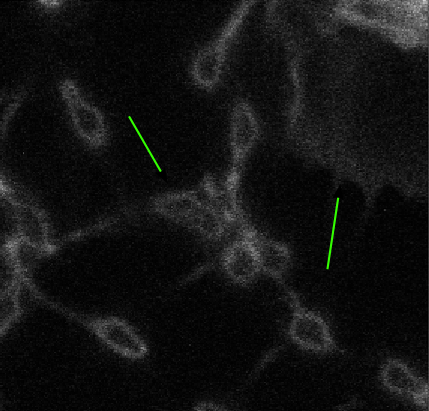
\includegraphics[width=0.6\linewidth]{resources/tmp/t017_upperright.png}
    \end{center}
    \caption{Subpart of the original data showing noise and artifacts.}
    \label{fig:upperright}
\end{figure}
It is still important to be able to somehow split the dataset into the training
and testing sets. As the dataset is rather sparse, choosing a random subset to
evaluate performance is not ideal, and there is a random chance that some tunnel
from the testing set may be visible in a cutout of a tunnel in the training set.
Another problem is how the various parts of the dataset do not have the same
number of tunnels, tunnels of the same morphology and the same amount of noise
and irrelevant structures. For example, in the upper right corner in Figure
\ref{fig:upperright} we can find some irrelevant structures which are not
present in the rest of the dataset. Given these problems, it is pretty tricky to
split the dataset in such a way that all possible types of artefacts and tunnel
structures are visible in both the testing and training subsets.

We tackled this problem by doing a quadrant-based spatial 4-fold
cross-validation. In each training run, one of the four quadrants is selected as
the testing quadrant, and all cropped TNTs belonging to this quadrant form the
testing subset. This helps mitigate the small dataset and enables us to study
how the different folds affect the performance of the neural network.

\begin{figure}
    \begin{center}
        \includegraphics[width=0.6\linewidth]{resources/dataset/vis_split_t0.png}
    \end{center}
    \caption{A visualisation of the division into a training and testing subset
    for one of the folds.}
    \label{fig:folding-visualisation}
\end{figure}

This is still quite challenging to do correctly, as not every tunnel lies neatly
inside one of the quadrants. A split used in training is visualised in Figure
\ref{fig:folding-visualisation}, where a possible split is shown in two colours:
red represents cutouts belonging to the testing subset. The decision of whether
a cutout belongs to the testing subset or not is dictated by looking at the
overlap with the training quadrant. If the crop lies with more than 20\% or has
more than 50 pixels in the testing quadrant, it will not be included in the
training subset. If at least 80\% of the cutout is inside the testing quadrant,
it is considered to be part of the testing subset.

Finally, during the training we need the be able to know when to stop. For this
purpose during each run, roughly 30\% of the crops used for training are used as
a validation set.

\section{Loss funtions}
Since we can look at finding tunneling nanotubes as a binary classification
problem applied at every pixel, it naturally comes to use a binary cross-entropy
loss to teach the network to learn to segment the images. However, our dataset
is very heavily imbalanced as the data contains a lot more negative examples. To
somewhat help the training to pay more attention to the tunnels, the
cross-entropy was weighted by a factor or 50, which was estimated by taking the
calculating the ration of pixels classified as background and pixels assigned to
some tunnel by the biologist. The weighted BCE loss is defined as
\parencite{Jadon2020loss} \parencite{PyTorchBCE}:

\[ L_{BCE}(y, \hat{y}) = -(\beta*ylog(\hat{y}) + (1-y)log(1-\hat{y}) \]

where $y$ stands for prediction, $\hat{y}$ is the true label, and $\beta$ is the
weight.

To further improve the performance of the training, we got inspired CS-Net paper
which uses Dice loss, and some papers claim that the combination of Dice loss
and cross-entropy loss lead to better performance in many segmentation tasks
\parencite{ma2020segmentationlossodyssey}. As Dice is a common metric to
evaluate segmentation performance it is  By using Dice loss it is meant to
optimize the value of the Dice coefficient. This is defined as taking $L_{Dice}
= 1 - \text{Dice}$, meaning that as we get segmentation results closer to the
ideal mask, we get closer to 0. The loss function was defined using as in the
paper \parencite{ma2020segmentationlossodyssey} as:

\[ L_{Dice}=1-\frac{2\sum_{i=1}^{N}{g_i*s_i}}{\sum_{i=1}^{N}{g_i^2}+\sum_{i=1}^{N}{s_i^2}} \]

where $g_i$ is the binary indicator for the foreground and $s_i$ is the
probability of assigning the pixel to the foreground class.

The final loss is the combination of $L_{BCE}$ and $L_{Dice}$:

\[ L_{final} = 0.5 L_{Dice} + 0.5 L_{BCE} \]

We used a linear combination of the losses as was mentioned in
\parencite{ma2020segmentationlossodyssey}.

During the development of the training loop, we observed that setting the
learning rate to 0.0001 and weight decay to 0.0001 provided a stable learning.
As such, we maintained a constant learning rate during training and did not
experiment with these values due to time constraints. We chose to use an
adaptive gradient algorithm for training the neural networks called AdamW, which
is a variant of the commonly used Adam optimiser.

\section{Optimisers, learning rates, regularisation}

Regularisation is a common technique in machine learning that reduces
overfitting by discouraging values with large magnitudes
\parencite{Bishop2024DeepLearning}. One of the standard regularisation
techniques in deep learning is weight decay, also known as L2 normalisation,
which penalises large weights [TODO check]. However, while L2 normalisation and
weight decay are the same, this is not true for the Adam optimiser. The authors
argue that using their version, called AdamW, achieves better generalisation
performance as it properly decouples the weight decay
\parencite{loshchilov2019}. Since we have a sparse dataset, we wanted to include
the weight decay regularisation technique. However, no significant difference in
the training performance was observed.

\section{Augmentations}

A common problem with training neural networks is their capacity to overtrain on
the training part of the dataset. This often leads to poor generalisation
performance. This is especially true for tiny datasets such as ours. One of the
common ways to address this problem, as mentioned in the original U-Net paper,
is the use of augmentations \parencite{Ronneberger2015} to artificially enlarge
the training set. In our case, we decided to use only augmentations that do not
require interpolation. The reason is that, unlike many other tasks, we are
potentially dealing with relatively thin structures, which could be easily
suppressed or blurred and no longer visible with improper interpolation.

In each batch, a different set of transforms is used. This works by setting a
random probability for this particular transform to be applied. For the training
we are:
\begin{itemize}
    \item{Adding random noise with a Gaussian distribution of mean 0 and 0.01
        standard deviation with probability 0.5, which adds very faint noise.
        This is a relatively low amount of noise and was chosen during the
        development of the network as we did not want to change the images to
        look completely different to the orignal ones.}
    \item{Random flipping in every axes.}
    \item{Random spatial crop which always crops to the preset size 7x64x64 from
        any other size.}
\end{itemize}
A possible problem of using small tiles centered at tunnels is that we might
introduce unwanted bias into the network, as it might learn to always try to
find the tunnel in the middle. The design designation behind using random
spatial crop was to try to suppress this, as the program now randomly finds a
crop of the wanted size, which reduces this problem.

\section{Training loop}
Overall the network training loop is shown in Algorithm \ref{alg:training}. Just
a note the evaluation here is just calculating the Dice score on top of the
crops belonging to the training quad.

\begin{algorithm}[H]
    \setlength{\lineskip}{-3pt}        % Reduce line spacing
    \setlength{\baselineskip}{8pt}      % Reduce baseline spacing
    \setlength{\parskip}{0pt}           % Remove paragraph spacing
    \small  
    \caption{Quadrant-based Model Training}
    \label{alg:training}
    \KwData{Four quadrants, model configuration}
    \KwResult{Four trained models}

\For{$quad \in quadrants$}{
    $Reseed()$\;
    
    \tcp{Data preparation}
    $full\_train\_data, full\_test\_data \gets LoadQuadrantData(quad)$\;
    $mean, std \gets ComputeStats(full\_train\_data)$\;
    $train_{set}, val_{set} \gets SplitData(full\_train\_data, ratio=1/3)$\;
    
    \tcp{Model training with early stopping}
    $model \gets CreateNeuralNetwork(config)$\;
    $best_{loss} \gets \infty$\;
    
    \For{$epoch \gets 1$ \KwTo $1000$ \textbf{or until} $val\_loss$ hasn't improved for 50 epochs}{
        $loss_{train} \gets TrainEpoch(model, train_{set}, mean, std)$\;
        $loss_{val} \gets ValidateEpoch(model, val_{set}, mean, std)$\;
        
        \If{$loss_{val} < best_{loss}$}{
            $best_{loss} \gets loss_{val}$\;
            $SaveBestWeights(model)$\;
        }
    }
    
    $LoadBestWeights(model)$\;
    $SaveFinalModel(model, quad)$\;
    $EvaluateModel(model, full\_test\_data)$\;
}
\end{algorithm}

\section{Inference on large images}

Our network has been trained on square crops of size 7x64x64 voxels, but the
original images are larger at 7x512x512 voxels. This is solved by using an
overlap-tiling strategy similar to the one by Ronneberger et al.
\parencite{Ronneberger2015}. The original images a re split into tiles first
with configurable amount of overlap in pixels, this is visualised in Figure
\ref{fig:tiling}. The tiles are sequentially processed by the network and then
stitched together to create the final prediction.

\begin{figure}
    \centering
    \begin{subfigure}[t]{0.5\textwidth}
        \centering
        \includegraphics[width=\textwidth]{resources/t000-3-0verlap.png}
        \caption{0px overlap}
        \label{fig:stitchingoverlap0}
    \end{subfigure}\hfill
    \begin{subfigure}[t]{0.5\textwidth}
        \centering
        \includegraphics[width=\textwidth]{resources/t000-3-30overlap.png}
        \caption{30px overlap}
        \label{fig:stitchingoverlap30}
    \end{subfigure}
    \begin{subfigure}[t]{0.5\textwidth}
        \centering
        \includegraphics[width=\textwidth]{resources/t000-3-orig-stretched.png}
        \caption{Original image (stretched).}
    \end{subfigure}
    \begin{subfigure}[t]{0.5\textwidth}
        \centering
        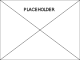
\includegraphics[width=\textwidth]{resources/placeholder.png}
        \caption{30px overlap with postprocessing} 
    \end{subfigure}
    \caption{This figure shows how choosing different amount of overlap in
    pixels has an effect on suppresing some of the artifacts at the borders of
    stitched tiles.}
    \label{fig:stitchingoverlap}
\end{figure}

The idea to use a configurable overlap size came from the following observation.
In Figure \ref{fig:stitchingoverlap0}, several sharp artefacts can be seen at
tile borders, possibly because only part of the structure is vissible, leading
the network to classify it as a tunnel. This led us to the idea that if we use
larger overlaps and aggregate them, these effects on tile borders will get
suppressed. As can be seen in Figure \ref{fig:stitchingoverlap30}, using a
larger overlap suppresses some of these artefacts. For aggregating the overlaps,
a simple averaging was chosen due to its simplicity

% todo in discussion mention that maybe this was not the best idea, maybe we
% should have chosen larger context. The context x precision tradeoff.

% TODO: consider drawing there
Even after this step, there still might be some leftover artefacts, some of
which are linked to noisy input, but others are showcase that is is not a
perfect solution to the artefacts caused by partial context. Some of these false
TNTs at the border of tiles are quite small compared to real tunnels, which
lead us to the final piece of the inference - the postprocessing.

\section{Postprocessing}
\label{sec:postprocessing}

As mentioned in the previous section, even after applying the overlap strategy,
some artefacts remain. Moreover, some artefacts actually closely resemble thin
structures but are not true tunnels. Many of these false tunnels seem to be
small and not connected to any cell, nor are significantly present at multiple
depth slices. Therefore, we decided that an easy filtering would be using their
volume.

\begin{figure}
    \begin{center}
        \includegraphics[width=0.6\linewidth]{resources/histogramofsizes.png}
    \end{center}
    \caption{Histogram of the volume (in pixels) of all labeled tunneling
    nanotubes with median and mean highlighted.}.
    \label{fig:histogramoflabelsizes}
\end{figure}

I chose the value of 100 pixels, realising that some of the tiny tunnels might
get removed, but as will later be shown, the network tends to find more tunnels
than the biologist. Hence, I believe this to be a reasonable assumption to make.
% todo: mention in discussion that this prob. could have been more studied

\chapter{Implementation}

\section{Used technologies}
Python, mlflow, Bash, uv, the shuffling, setting explicit seeds, issues with
batch vs loss, implementing the loss functions in pytorch
implementing the squeeze and excitation.

\section{Environment}

\subsection{Justification for the used technologies}
The previously described training and preprocessing in previous chapters was
implemented as collection of Bash scripts, python scripts and a python module.
All of the code is available as part of the master thesis alongside several of
the trained networks for the user.

The Python environment is packaged and its dependecies are resolved by a tool
cold uv \parencite{uv} developed by a company called Astral, who specialises on
creating modern automatic tooling for Python. The environment is described using
a TOML file available and list a number of dependencies. Altough the project is
quite recent compared to others like Poetry, uv is significanlty faster.

For convenience I am also including a \texttt{requirements.txt} which was automatically generated
from a virtual Python environemnt, but the officially supported version is using
the uv package manager. The environment can then be created in two ways: if the
user runs a computer with a GPU, the working environmnet is creating using the
command \texttt{uv sync --extra torch-gpu} which assumes that CUDA version 12.4
is installed.

I decided to use Python to develop the training and evaluation scripts, while
handling the pipelines around it with Bash. Altough Python is an interpreted and
dynamically typed language and therefore is comparably slower than other lower
level languages traditionally used in image processing like C++, its nature
allows it to rapidly prototype new application. Moreover, many packages call
code written in other languages such as C++, Fortran or C, to somewhat alleviate
the performance problem. Lastly, Python has become a widely adopted language in
the area of neural networks, and many researchers publish their code in Python.

As was already mentioned even though the majority of code is written in Python
it is quite cumbersome to create a single Python script which handles both
training and evaluation, especially if something changes in one of them. This
fundamentally breaks the famous principle in software architecture called the
separation of concers. As such a bash script is provided in the code archive
under \texttt{scripts} called \texttt{run.sh} which is the main entrypoint for
running the code.

As a lot of the evaluation is concerned with doing proper cross-validation and
then averaging the results it was easier to create a script which is easily
configured using a text editor or by providing and parsing CLI arguments and the
averaging and choosing different datasets should not be a responsibility of the
Python script. As such, creating directories, running code, aggregating results
and parsing arguments is a natural job for a scripting language such as Bash.
The obvious disadvantage is that it is limited to the Unix and Unix like
operating systems.

As for the other tooling, here I list the most important tools:
\begin{itemize}
    \item{MLflow is tool for handling machine learning pipelines, it allows to
        track experiments, compare results, save and load models, deploy models
        etc. In this work it was used to create a nice interface to keep track
        of various experiments.}  % cite https://mlflow.org/docs/latest/ml/
    \item{ruff linter TODO cite is an extremely fast Python linter which was
        developed by the company Astra. It automatically formats code and can
        even fix some of the basic lint errors.}
    \item{numpy TODO CITE has become one of the fundamental packages in
        scientific computing in Python ecosystem. It provides a very efficient
        implementation of} 
    \item{scikit-learn provides a great framework for building machine learning
        models not just deep learning models. This was used mainly for splitting
        datasets and using their framework for handling batching.}  % TODO: https://scikit-learn.org/stable/index.html
    \item{scikit-image is a package providing various algorithms for processing
        images e.g. segmentation algorithms, point transform, mathematical
        mopohlogy. I used it to handle the post-processing of masks and to find
        connected components.} % TODO: https://scikit-image.org/
    \item{Pytorch is a popular deep learning framework with focus on flexibility
        and speed, this allows the user to create a well performing neural
        network very fast. It automatically creates computational graphs
        allowing it to compute gradient upgrades efficiently. It handles
        connecting to various hardware like CPU and GPUs automatically. This has
        allowed PyTorch to become one of the most used packages in the Python
        ecostsem and is why I chose it to develop the program. TODO CITE} % https://pytorch.org/projects/pytorch/ 
    \item{MONAI is another opensource framework for building neural networks on
        top of PyTorch. It focuses on building models used in Medical area. In
        the project I was using this package to handle augmentations of the
        dataset as it provides first class support for 3D data.} % cite https://github.com/Project-MONAI/MONAI
    \item{matplotlib}
\end{itemize}

\section{Use case modelling and expected usage}
Here describe how to call the run.sh
We identified two particular use cases for the application, it should provide a
reasonably easy interface for training and then an interface for evaluating the
models given some training data. For this purpose a single Bash script called
wasc created which serves the 

\chapter{Evaluation}
In this chapter we describe how and evaluate the different networks on the whole
dataset and how a study on the depth and overlap was done.

\section{Metrics}
For evaluating the resulting predictions we decided to use Dice scores as they
are commonly used in many biomedical papers [TODO citation needed] but the end
user is not interested in the quality of the scores on cutouts around tunnels,
instead we must somehow use our neural network for predicting over the whole
images. For this purpose, we will present the Dice scores calculated using the
stitched predictions as described in Section \ref{sec:runningthenetwork}. In
these cases the labels are binarised, and with the binary prediction mask, the
final score is calculated. Similarly, this is done with the postprocessed
images. These numbers are by itself important, but we would also like to
investigate how the network does on the level of tunnels and in terms of how
well does it segment tunnels which are really present as compared to faint
artefacts.

\subsection{Mapping}
\label{sec:mapping}
It is obviously important to calculate Dice on the whole images for
the final evaluations, but is it sometimes quite important to also see how well
the network segments tunnels is correctly identifies. For this purpose we
developed the following extra metrics.


\begin{figure}
    \centering
    \begin{subfigure}[b]{0.45\textwidth}
        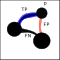
\includegraphics[width=\linewidth]{resources/inkscape/matching_simple.png}
        \caption{}
        \label{fig:matchingsimple}
    \end{subfigure}
    \hfill
    \begin{subfigure}[b]{0.45\linewidth}
        
\includegraphics[width=\linewidth]{resources/inkscape/matching_multiple.png}
        \caption{}
        \label{fig:matchingmultiple}
    \end{subfigure}
    \caption{An example of three vertical pillars (black circles) and tunnels
    (in black)
    connecting them. In Subfigure \ref{fig:matchingsimple} we can see one good
    prediction and one false one. In SubFigure \ref{fig:matchingmultiple} we can
    see a single large prediction covering both tunnels.}
    \label{fig:matchingdiagram}
\end{figure}

The way we have defined specially look at tunnels which were correctly
identified and see how well the network worked in segmenting them out. In Figure
\ref{fig:matchingsimple} we can see a simple hypothetical schematic of a
situation in which a we have three vertical pillars, shown here as three black
circles, and two tunnels connecting them, here the tunnels are in black. Now the
neural network might predict multiple connected components, but only some of
them are right matches and correspond to a tunnel. In this figure, it is okay to
say that the blue tunnel is predicting one of the true tunnels, albeit it is
little bit oversegmenting the tunnel. On the other hand, the red prediction is
completely off and it is not connected to any underlying tunnel; therefore, this
should be counted as a false predictions.

As we look into the data we might see that often time the tunnels, especially in
places where there a cluster of tunnels might not be perfectly separated. They
may be touching or even crossing each other. In some cases two tunnels visually
look like they have joined together. In this cases if we picked the strategy in
\ref{fig:matchingsimple} where predictions and labels are matched according to
the closest match, we would severally penalise predictions which touch. This is
a problem as it is weird to penalise the network if single predicted component
covers multiple predictions. The problem is again schematically visualised in
Figure \ref{fig:matchingmultiple}, where a tunnel prediction in blue, matches
two different tunnels in black). I would argue that it is unfair to penalise the
metrics in this case.

This idea is technically implemented in the following manner inside the
evaluations. We take the predictions of the neural networks and calculate the
component components in 3D. As described previously, the components are filtered
by size and thresholded. Now comes the matching. In the first pass the
application will iterate over all labels in the ground truth and see if there
are any predictions which contain at least 50\% of the mask. All of these
matches are then accumulated. In the implementation and further diagrams we
refer to this as all matches. The value 50\% was chosen so that a single ground
truth label cannot be contained in multiple predicted connected components.

Now that we have assigned possible multiple labels to each predicted connected
component we can divide the mapping into what is referred to as clean matches
and all matches. In Figure \ref{fig:bipartitematching} we see a diagram of an
example of a possible matching. In these case the network predicted three
tunnels, and the data has three labeled tunnels. In this case a predicted tunnel
denoted as $p_1$ is uniquely mapped to label $l_1$. Since $p_1$ is not connected
to any other label, we call this a clean match. On the other hand predicted
connected component $p_2$ has according to the aforementioned algorithm been
mapped to two different labels $l_2$ and $l_3$. As previously argued it would be
unwise to disregard this mapping as a bad one, therefore we will also accept
this mapping and it will show up in following metrics when we refer to all
matches.

Finally, this allows us to quantify how well different networks understand the
image not on a pixel by pixel manner, but in terms of the whole tunnels. We can
look at the prediction $p_3$ as a false positive, since it is not mapped to any
tunnel, while the label is $l_4$ is viewed as a missed tunnel, and therefore
called a false negative. All clean matches ($p_1$->$l_1$) are considered to be a
true positives, while multiple matches are, according to the precious arguments,
also considered as a true positive, in fact this is counted as a single true
positive.

To summarise, we are going to look at the Dice score for the following cases:
\begin{itemize}
    \item{Test: In this case we are looking at performance on cutouts of tunnels
        in one particular quadrant}
    \item{Evalution: In this case we are calculating the performance from the
        overall stitched binary images.}
    \item{Postprocesed overall: In this metric, the postprocessing described in
        Section \ref{sec:postprocessing} is applied on top of the predictions,
        and whole images are evaluated}
    \item{Postprocessed Clean matches: In this metric, we overlay the binary
        masks of cleanly matched tunnels and predictions and calculate the Dice
        score.}
    \item{Postprocessed all matches: Like above, but even predictions mapped to
        multiple labels are used.}
    \item{Tunnel metric: Here we care about just the mapping described in Figure
        \ref{fig:bipartitematching}}
\end{itemize}
% todo: definitely deserves more attention
% todo: as an example, show the quad with all sort of tunnels connected together
% todo : btw am i explainign the how we binarise the labels?

\begin{figure}
    \begin{center}
        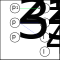
\includegraphics[width=0.4\linewidth]{resources/inkscape/matching_bipartite.png}
    \end{center}
    \caption{A diagram showing how multiple }.
    \label{fig:bipartitematching}
\end{figure}

Lastly, to reiterate the idea presented in the training Section [TODO: not
written yet], we are always training the network on three of the four possible
quadrants. As such, four different models are always trained and the results
will averaged.

\section{Ablation studies}
In this section we will present experimentally inferred sizes of hyperparameters
for the neural network.

\subsection{Choice of depth and overlap for the network}
\label{sec:ablation-depth}
While working on the network the choice of depth and overlap is not obvious, but
it is a very important parameter as every advanced architecture is build on top
of the anisotropic unet described in Chapter [TODO], which has customizable
depth. Moreover, the reason why the anisotropic version was created is to allow
us to change the depth.

In general it is accepted that the ability to teach deeper network helped improve
neural networks performance and in some sense, the ability to teach deeper
networks lead us to the neural network revolution. [TODO cit. needed] % TODO citation needed
But, the size of the network should be somehow connected to the
complexity of the problem, both in terms of size of the context and the image
complexity. To find a reasonable value for this parameters we decided to do a 2D
hyperparameter search study. 
% todo: talk about this in the discussion

We took the 3D version of the Anisotropic architecture (AnisoUNet3D) and
considered five different versions. The shallowest one has exactly two
downsampling layers --- so it is referenced as a network with depth equal to 2
--- and the deepest one has 6 downsampling layers. Six downsampling layers was
chosen as this is enough to reduce the original size 7x64x64 to 7x1x1 as such,
there is no need to have a deeper network.

For the overlap hyperparameter we chose the values 0px, 10px, 20px, 30px, and
40px. The value 40px was chosen arbitrarily, as in this case, the neighbouring
cells already share more than half of the volume.

As the overlap is a hyperparameter of the postprocessing, this means that only
five different architectures must be trained to perform this analysis. Since we
are doing cross fold analysis, we are training 20 models. Finally, since neural
networks employ randomness, each combination of fold and architecture is
repeated three times, leading to training 60 models for this evaluation.

The Figure \ref{fig:parametersearchstudy} showcases the dice score of the
various networks. Every number is the mean performance across the 4-cross fold
validation and 3 independent runs i.e. an average of 12 networks. Overall the
highest number is highlighted and it corresponds to the version with three
downsampling layers and 10px overlap; thus, all following models will be using
this combination of hyperparameters.
% TODO: tripple check, i had very different numbers before

\begin{figure}
    \begin{center}
        \includegraphics[width=0.8\linewidth]{resources/evaluations/eval_dice_mean_heatmap.png}
    \end{center}
    \caption{Evaluation Dice score for various depths of the network. Best
    values is highlighted.}
    \label{fig:parametersearchstudy}
\end{figure}


What we can also see from this hyperparameter search is that the effect of
number of downsampling layers is rather marginal and there is not a clear trend
of more downsampling layers leading to better performance or vice-versa. Another
effect that is visible is that while changing between 10 pixels to 20 or 30
pixels does minimal change in the performance, the difference between 0 pixels
and all others is visible in every case. Also it is interesting to see, that
although the changes are not greatly different, the network with three
downsampling layers seems to always beat the others.

For further studies, we took a look at just 10 pixel overlap and looked at other
metrics, which were introduced in the previous chapters. In Figure
\ref{fig:eval:depth} the effect of the depth is studied more. I chose three
different metrics to investigate the effect of postprocessing and the
performance on the level of tunnels. Just to make clear, in these graphs, each
average is calculated as the mean of the performance across four cross folds
and three runs. The error bars are +- a single sample standard deviation of
these values.

First of all, it is visible, that the performance differences across various
depths is not that significant, but overall the network with three downsampling
steps and the network with five downsampling steps are achieving consistently
the highest averages, while the networks with two and six downsampling steps are
performing the worst. I believe this can be explained by the fact, that the
deepest network is unreasonable large for our given problem, while the smallest
network might suffer from not enough layers.

However, it must be noted, that the error bars are very large and complicate any
conclusion, as it shows that the performance varies quite dramatically. This
lead us to investigate what could be causing this variety, and one possible
explanation is the various performance on the quadrants.

Taking a look at Figure \ref{fig:eval_quads} here we can see the same metrics,
but this time it is further divided among the various quadrants. What is
immediately obvious us that the error bars are less varied, due to the
performance differences across quadrants. Interestingly, in some cases like the
models with 6 downsampling layers for the first quadrant has large performance
differences, but no reason as to why this happens was found. Since in this case
all bars are averages of three numbers, it is plausible that due to bad luck,
sometimes the network does not achieve as good of a performance as in other
runs. % TODO talk in discussion

In general, all models performed the best at the first quadrant (top left) and
third quadrant (bottom left), while the performance was lower on the second
quadrant (top right) and the fourth quadrant (bottom right). Looking at the
means and error bars now, it seems that the model with three downsampling layers
performs best or close to best in all folds, while having more layers can
sometimes reach similar performance it might also lead to worse (like in case of
three downsampling steps in quadrant 3); hence, we cannot say that for our input
size, the increased depth helps dramatically. But our previous decision to
choose the network of depth three in the following studies still stands, as even
tough the performance difference is not that different, this network is
consitently beating the smaller network and at the same time has much less
parameters than the larger networks.

\begin{figure}
    \centering
    \begin{subfigure}[b]{0.8\textwidth}
        \centering
        \includegraphics[width=\linewidth]{resources/evaluations/eval_dice_mean_architecture_comparison.png}
        \caption{Evaluation performance.}
        \label{}
    \end{subfigure}\hfill
    \begin{subfigure}[b]{0.8\textwidth}
        \centering
        \includegraphics[width=\linewidth]{resources/evaluations/postprocess_overall_dice_architecture_comparison.png}
        \caption{Performance with post-processing.}
    \end{subfigure}
    \begin{subfigure}[b]{0.8\textwidth}
        \centering
        \includegraphics[width=\linewidth]{resources/evaluations/tunnel_dice_architecture_comparison.png}
        \caption{Performance on tunnels.}
        \label{fig:eval-depth-tunnels}
    \end{subfigure}
    \caption{Performance evaluations of the neural networks for various depths
    and fixed 10 pixel overlap.}
    \label{fig:eval:depth}
\end{figure}

\begin{figure}
    \centering
    \begin{subfigure}[b]{0.8\textwidth}
        \centering
        \includegraphics[width=\linewidth]{resources/evaluations/eval_dice_mean_by_quad_arch.png}
        \caption{Evaluation performance.}
    \end{subfigure}\hfill
    \begin{subfigure}[b]{0.8\textwidth}
        \centering
        \includegraphics[width=\linewidth]{resources/evaluations/postprocess_overall_dice_by_quad_arch.png}
        \caption{Performance with post-processing.}
    \end{subfigure}
    \begin{subfigure}[b]{0.8\textwidth}
        \centering
        \includegraphics[width=\linewidth]{resources/evaluations/tunnel_dice_by_quad_arch.png}
        \caption{Performance on tunnels.}
        \label{subfig:eval_tunnels}
    \end{subfigure}
    \caption{Performance evaluations of the neural networks for various depths
    and fixed 10 pixel overlap.}
    \label{fig:eval_quads}
\end{figure}

\subsection*{Different architectures}
\label{sec:diff-architectures}
As we have discussed in the previous section, we did a 2D hyperparameter search
to choose a good estimate of the depth and overlap values, since these are used
by our advance neural networks, we picked 3 downsampling layers and an overlap
of 10 pixels. In this section the evaluation of other networks will be
presented.

We decided to study the following architectures: a basic implementation of UNet
as described in Section [TODO]. Its anisotropic version as described in Section
[TODO], a version of Anisotropic model with the CSAM module as described in
Section \ref{sec-csammodule}, and finally the UseNet architecture from Section
\ref{sec-seblock}. All models are using 10 pixel overlap and their depth is
equal to three downsampling blocks, with the exception of BasicUNet, which has
two downsampling blocks.

Moving on to the results Figures \ref{fig:eval-diff-arch-dice}-
\ref{fig:eval-diff-arch-tunnel} shows the same metrics we discussed in Section
\ref{sec:ablation-depth} aggregated across all the cross folds, while
\ref{fig:eval-diff-arch-dice-quads}-\ref{fig:eval-diff-arch-tunnel-quads} shows
the performance for each quadrant. The means and standard derivations of all
metrics was calculated exactly the same as in the previous section, again every
combination was trained three times.

We can again see a similar pattern with the large error bars in all figures
especially the Figure \ref{fig:eval-diff-arch-tunnel} when looking at the tunnel
metrics. Of note is that the BasicUNet architecture is performing worse than all
others in every metric even accounting for the standard derivation.

As such, the problem of large discrepancy in performance is similarly caused by
different performance across the folds, where the overall dice performance is
highest for the third quadrant while being relatively lower for the second
quadrant and fourth quadrant in Figure
\ref{fig:eval-diff-arch-dice-overall-quads}.

While it is difficult to asses the overall trends due to the error bars, an
interesting observation is that the 2D versions tend to perform equally like in
third quadrant in Figure \ref{fig:eval-diff-arch-dice-overall-quads} or slightly
better than their 3D versions. I suspect this could be caused by having
significantly less parameters compared to the 3D versions.

Since the error bars are quite large even tough the value is calculated from 12
values for each bar, it would be insightful to find out what causes this.
Inspired by the previous hyperparameter search section, additional graphs, where
the performance is analysed per quadrant were created in Figures
\ref{fig:eval-diff-arch-dice-quads}-\ref{fig:eval-diff-arch-tunnel-quads}.

In Figure \ref{fig:eval-diff-arch-dice-quads} the overall evaluation dice is shown
and in Figure \ref{fig:eval-diff-arch-dice-overall-quads} are results with the
postprocessing applied. Looking at the dice results it is clear that the
postprocessing neealy always helps increase the metric's value, but it is rather
on the second decimal position. And the effect is largest on the third quadrant.

If we were to just focus on the nicely segmented tunnels i.e. those that were
matched we can see that the overall dice score jumps to higher values, reaching
even around 0.68 in the second quadrant. Hence, it looks like the overall Dice
score is being lowered by false predictions, which even the postprocessing is
not able to remove.

Lastly, we will talk about the Dice score on the level of tunnel detection as
was described in Section \ref{sec:mapping}. Compared to the overall Tunnel
scores in Figure \ref{fig:eval-diff-arch-tunnel-quads}, where it seemed according to
the average values, that the 2D version have slight advantage, here it is not so
clear, there also seems not be any clear clearly better architecture than the
rest.


\begin{figure}
    \begin{center}
        \includegraphics[width=0.9\linewidth]{resources/evaluations/diffarchs/eval_dice_mean_architecture_comparison.png}
    \end{center}
    \caption{dice}
    \label{fig:eval-diff-arch-dice}
\end{figure}
\begin{figure}
    \begin{center}
        \includegraphics[width=0.9\linewidth]{resources/evaluations/diffarchs/postprocess_overall_dice_architecture_comparison.png}
    \end{center}
    \caption{overall dice}
    \label{}
\end{figure}
\begin{figure}
    \begin{center}
        \includegraphics[width=0.9\linewidth]{resources/evaluations/diffarchs/postprocess_clean_matched_dice_architecture_comparison.png}
    \end{center}
    \caption{dice on cleaned matches}
    \label{}
\end{figure}
\begin{figure}
    \begin{center}
        \includegraphics[width=0.9\linewidth]{resources/evaluations/diffarchs/postprocess_matched_dice_architecture_comparison.png}
    \end{center}
    \caption{dice on all matches}
    \label{}
\end{figure}
\begin{figure}
    \begin{center}
        \includegraphics[width=0.9\linewidth]{resources/evaluations/diffarchs/tunnel_dice_architecture_comparison.png}
    \end{center}
    \caption{dice on tunnel level}
    \label{fig:eval-diff-arch-tunnel}
\end{figure}


\begin{figure}
    \begin{center}
        \includegraphics[width=\linewidth]{resources/evaluations/diffarchs/eval_dice_mean_by_quad_arch.png}
    \end{center}
    \caption{eval dice}
    \label{fig:eval-diff-arch-dice-quads}
\end{figure}
\begin{figure}
    \begin{center}
        \includegraphics[width=\linewidth]{resources/evaluations/diffarchs/postprocess_overall_dice_by_quad_arch.png}
    \end{center}
    \caption{overall dice}
    \label{fig:eval-diff-arch-dice-overall-quads}
\end{figure}
\begin{figure}
    \begin{center}
        \includegraphics[width=\linewidth]{resources/evaluations/diffarchs/postprocess_clean_matched_dice_by_quad_arch.png}
    \end{center}
    \caption{clean matched}
    \label{fig:eval_diff_arch_clean_match_dice_quads}
\end{figure}
\begin{figure}
    \begin{center}
        \includegraphics[width=0.8\linewidth]{resources/evaluations/diffarchs/postprocess_matched_dice_by_quad_arch.png}
    \end{center}
    \caption{matched dice}
    \label{fig:eval_diff_arch_matched_dice_quads}
\end{figure}
\begin{figure}
    \begin{center}
        \includegraphics[width=0.8\linewidth]{resources/evaluations/diffarchs/tunnel_dice_by_quad_arch.png}
    \end{center}
    \caption{tunnels}
    \label{fig:eval-diff-arch-tunnel-quads}
\end{figure}

\section{Recommended values}
As was discussed in the previous sections using the hyperparameter study and 

\chapter{Discussion and conclusion}
% what to do next
% talk about:
% - stitching x overlap size x size
% - recall threshold
% - size of network connected to the complexity
% - performance differences due to luck
% - myabe mention that the neural network could be trained using semi-supervised
%   approach?

% what could be done
% - 
In this work we took on a journey to investigate the feasibility of using
U-Net-like neural networks for segmenting nanotubular structures. Facing a very
sparsely labeled dataset of just two images we were able to train several neural
networks with various depths and attention mechanism. This was achieved through
the use of cross-fold learning and training the network on just cutouts of the
data where the tunnels were present.

Given the sparse annotations we were unable to explore how the different cutout
sizes influence the need for more complex network with deeper layers. In the
future another interesting topic would be to explore how the results could be
post-processed to further cleanup unwanted artefacts in the predictions.

Nevertheless, given the cirmustances and sometimes imperfect labels the neural
networks can be used to find predictions which are meaningful, even if the
network has a tendency to oversegment and flag various protrusion as false
tunnels with the correctly matched tunnels having Dice scores of around 0.6-0.7.
Mutltiple architectures with various attension mechanism were explored and shown
to provide small improvements on certains quadrants, but unfortunately no
architecture was found to have the best performance compared to the others.

As such the current implementation can be easily used by any machine equiped
with a GPU and the inference code deals automatically with the tiling and
stitching providing an easy to use interface for the user.


\end{document}
